\subsection{CET-STGL Representation and Evaluated Instantiation}
\label{sec:methodology}

\subsubsection{Overview}
CET-STGL is a causal-inspired event-token spatio-temporal representation framework for structured cellular operations data. It contains five feature blocks: KPI patch features, alarm event features, cell/time positional features, an event influence prior and inferred cross-cell context. Representation construction is separated from the downstream learner: heterogeneous signals are first aligned to the same cell-time-horizon index and then passed to forecasting, classification or prioritization heads. We evaluate a lightweight sklearn-based instantiation to isolate the utility of KPI patching, sparse event encoding, temporal context, train-only influence priors and inferred cross-cell information under a leakage-controlled protocol.

\noindent\textbf{Reliability-oriented representation principle.}
The design follows three constraints. KPI histories are summarized as local level and slope patches, sparse alarms are encoded by counts, decayed intensity and train-only association priors, and cross-cell context is inferred from training-period operational correlations when topology is unavailable. Compared with simple feature concatenation, CET-STGL imposes an explicit prediction-time constraint on each $(c,t,h)$ target, treats alarms as temporally weighted event context rather than raw indicators, and uses one admissible cell-time representation across forecasting, weak degradation classification and weak alarm-candidate prioritization.

\noindent\textbf{Temporal admissibility.}
For any prediction target at $(c,t+h)$, the evaluated CET-STGL feature vector is a function only of the lookback window $\mathcal{W}_{c,t}$, identifiers and time features available at $t$, and statistics fitted on the chronological training partition. No validation/test labels, post-$t$ observations or future event information are used in feature construction.

\noindent\textit{Justification.}
KPI patch features, alarm counts and decayed intensities are computed within $\mathcal{W}_{c,t}$. Degradation thresholds, feature scalers, event lifts and cross-cell graph statistics are estimated from the training partition only, and windows crossing the long time discontinuity are excluded before model fitting. The admissibility statement therefore concerns leakage-controlled representation construction, not causal identification or performance optimality.

The model structure and the evaluated lightweight implementation are summarized in Fig.~\ref{fig:cet_stgl_architecture}.

\begin{figure}[!t]
    \centering
    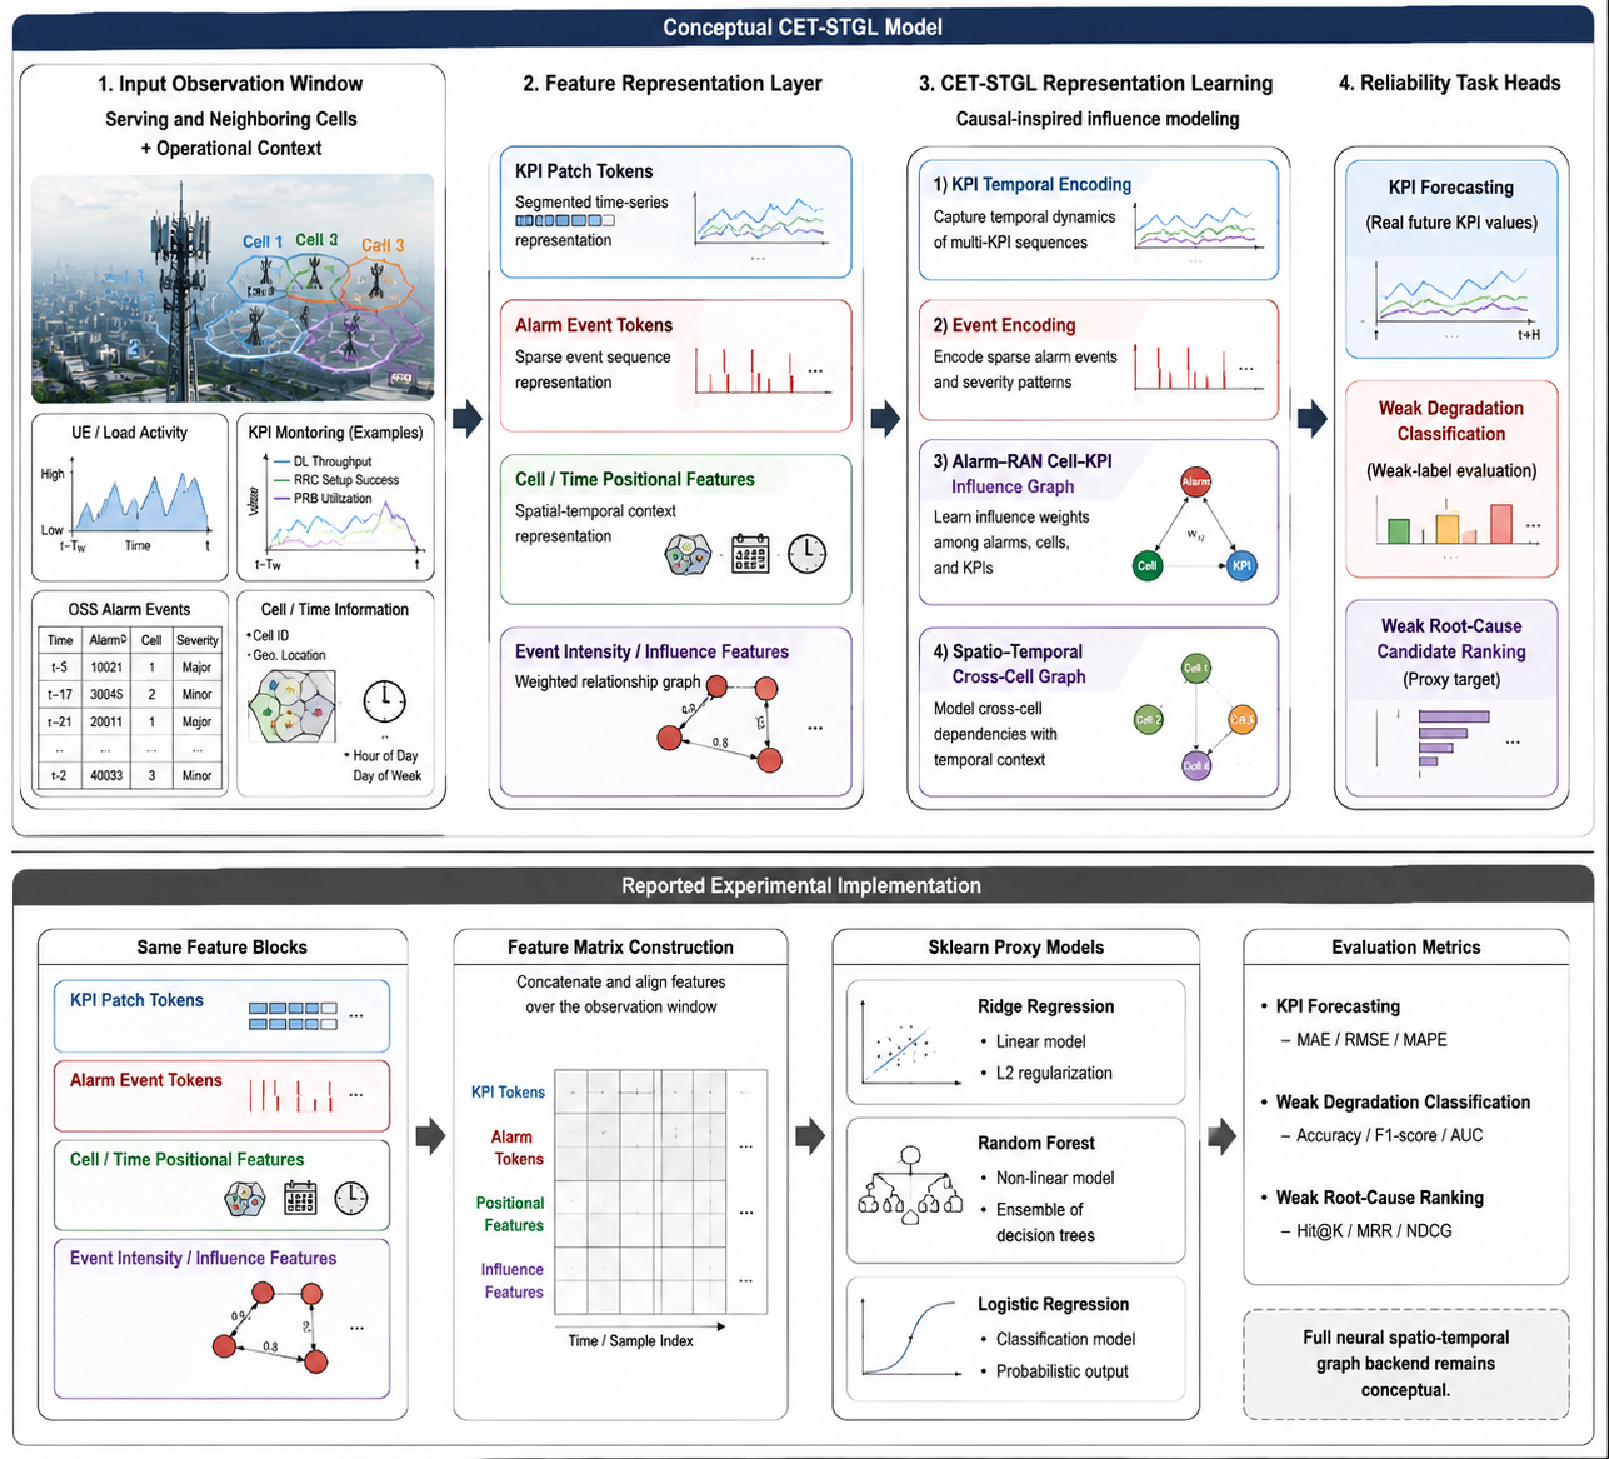
\includegraphics[width=0.98\textwidth]{figures/Fig_cet_stgl_model_architecture.pdf}
    \caption{Conceptual structure of CET-STGL, transforming heterogeneous cellular telemetry into event-aware spatio-temporal representations with influence modeling and a lightweight sklearn-based implementation for evaluation.}
    \label{fig:cet_stgl_architecture}
\end{figure}

\subsubsection{KPI Patch Features}
For each KPI $m$ in a lookback window, the sequence $x^{(m)}_{c,t-L+1:t}$ is divided into short patches. Each patch is summarized by simple local statistics:
\begin{equation}
    \phi^{\mathrm{kpi}}_{c,t,p,m}=
    [\mathrm{mean},\mathrm{slope}]_{c,t,p,m}.
\end{equation}
The patch summaries preserve local temporal level and slope while reducing raw sequence length. Patch-based features also support the multi-column KPI/business schema because all KPI columns can be transformed through the same compact local temporal summarization rule.
Patch-based time-series modeling provides a direct precedent for representing long temporal windows through compact local segments \cite{nie2023patchtst}.

\subsubsection{Alarm Event and Intensity Features}
Alarm/fault observations are represented as sparse event features. For alarm type $a$, we compute rolling counts and a decayed event intensity
\begin{equation}
    \lambda_a(c,t)=\sum_{\tau \leq t} \mathbf{1}[a_{c,\tau}>0]\exp\left(-\frac{t-\tau}{\eta}\right),
\end{equation}
where $\lambda_a(c,t)$ is the decayed event intensity for alarm type $a$ at cell $c$ and time $t$, $\mathbf{1}[a_{c,\tau}>0]$ is the binary indicator of the active alarm event at time $\tau$, and $\eta$ is a fixed decay scale in the feature implementation. The term Hawkes-inspired refers to the recency-weighted form, in which recent events contribute more strongly than older events \cite{hawkes1971spectra,mei2017neuralhawkes}. In the evaluated implementation, the decayed intensity is used as a fixed event feature rather than a fitted multi-type point-process model. Fixed decayed intensity matches the observed alarm sparsity: only 11 of 137 alarm/fault columns are active and only 1.62\% of rows contain an active alarm.

\subsubsection{Cell and Time Positional Features}
Cell identity and time context are encoded through cell-code features and cyclical time features such as hour-of-day and day-of-week. Cell and time positional features capture persistent cell offsets and periodic operational behavior. All transformations are fitted within the chronological training protocol, and windows crossing the detected long time gap are excluded.

\subsubsection{Train-Only Event Influence Prior}
For each alarm type and horizon, the evaluated instantiation estimates a train-only lagged lift:
\begin{equation}
    \mathrm{lift}_h(a)=
    \log\frac{P_{\mathrm{train}}(y_{c,t+h}=1 \mid a \in \mathcal{W}_{c,t})+\epsilon}
    {P_{\mathrm{train}}(y_{c,t+h}=1)+\epsilon},
\end{equation}
where $\mathrm{lift}_h(a)$ is the calculated lift value for alarm $a$ at horizon $h$, $P_{\mathrm{train}}$ denotes the probability estimated within the training set, $y_{c,t+h}$ is the target degradation label, $\mathcal{W}_{c,t}$ represents the lookback window, and $\epsilon$ is a small smoothing constant. The lift is combined with recent intensity to create event influence features. The event influence prior encodes temporal association between alarms and weak degradation using training data only. The prior is causal-inspired and leakage-controlled; it does not estimate a causal effect.

\subsubsection{Inferred Cross-Cell Graph}
The evaluated panel does not include verified physical topology. We infer a cross-cell context graph from training-period statistics, such as KPI correlation. Let $G_{\mathrm{cell}}=(\mathcal{C},E)$ denote the inferred graph. Neighbor features summarize KPI context from cells linked to $c$ in $G_{\mathrm{cell}}$. The inferred graph is a statistical context graph, not a physical deployment graph.
Training-derived cross-cell context follows the broader idea of using graph structure or adaptive spatial dependencies for time-series forecasting, while remaining explicitly statistical in the present dataset \cite{li2018dcrnn,wu2019graphwavenet}.

\subsubsection{Prediction Heads}
The evaluated instantiation uses sklearn-compatible heads: Ridge regression for multi-output KPI forecasting, a linear logistic classifier trained using stochastic gradient descent for weak degradation classification, and event-lift/intensity scoring for weak alarm-candidate prioritization. End-to-end neural spatio-temporal graph evaluation remains future work under the same leakage-controlled protocol.

